% GigaScience Technical Note - OmicsLake
% Template following GigaScience author guidelines
\documentclass[11pt,a4paper]{article}

% Packages
\usepackage[utf8]{inputenc}
\usepackage[T1]{fontenc}
\usepackage{lmodern}
\usepackage{microtype}
\usepackage{graphicx}
\usepackage{booktabs}
\usepackage{longtable}
\usepackage{array}
\usepackage{multirow}
\usepackage{hyperref}
\usepackage{xcolor}
\usepackage{listings}
\usepackage{amsmath}
\usepackage{amssymb}
\usepackage[margin=2.5cm]{geometry}
\usepackage[numbers,square,sort&compress]{natbib}
\usepackage{authblk}
\usepackage{lineno}
\usepackage{float}

% Line numbers for review
\linenumbers

% Hyperref setup
\hypersetup{
    colorlinks=true,
    linkcolor=blue,
    filecolor=magenta,
    urlcolor=cyan,
    citecolor=blue
}

% Code listing style
\lstset{
    basicstyle=\ttfamily\small,
    breaklines=true,
    breakatwhitespace=false,  % Allow mid-word line breaks to prevent overflow into margins
    columns=flexible,          % Maintain monospace appearance
    keepspaces=true,           % Preserve spaces exactly
    frame=single,
    language=R,
    showstringspaces=false,
    keywordstyle=\color{blue},
    commentstyle=\color{green!50!black},
    stringstyle=\color{red!50!black},
    literate={_}{{\_}}1        % Preserve underscores in identifiers
}

% Title
\title{OmicsLake: Versioned Data Management with Automatic Lineage Tracking for Reproducible Bioinformatics}

% Authors
\author[1,2,*]{Yusuke Matsui}
% Add co-authors as needed
% \author[3]{Second Author}

% Affiliations
\affil[1]{Institute for Glyco-core Research (iGCORE), Nagoya University, Nagoya, Japan}
\affil[2]{Biomedical and Health Informatics Unit, Graduate School of Medicine, Nagoya University, Nagoya, Japan}
\affil[*]{Corresponding author: matsui.yusuke.d4@f.mail.nagoya-u.ac.jp}

\date{}

\begin{document}

\maketitle

% ============================================================================
% ABSTRACT
% ============================================================================
\begin{abstract}
\noindent
\textbf{Background:}
Reproducibility in bioinformatics is often compromised by weak traceability of intermediate data states. Typical RNA-seq and multi-omics workflows iteratively transform data through normalization, filtering, modeling, and enrichment analysis, but these transitions are usually tracked manually. Code version control addresses scripts, not evolving analytical datasets. As a result, reconstructing the exact data state used for a specific result remains difficult in routine exploratory analysis.

\noindent
\textbf{Findings:}
OmicsLake is an R package for snapshot-oriented data-state management with automatic dataset-level lineage capture in dplyr workflows. The implementation combines DuckDB (primary local persistence and query execution), Apache Arrow (in-memory interchange), and Parquet (export/interchange format). Core operations are exposed through a compact API (\texttt{put}, \texttt{get}, \texttt{snap}, \texttt{restore}, \texttt{tree}) designed for low-friction integration into existing analyses. In benchmark settings aligned with submitted figures, OmicsLake showed faster import, aggregation, and join operations than representative baseline R workflows, while snapshot creation was slower than a file-copy proxy due to explicit in-database backup materialization.

\noindent
\textbf{Conclusions:}
OmicsLake achieved 100\% observed restoration success in RT-001 (30/30 iterations; 95\% CI: 0.88--1.00) using strict structural and numerical equivalence checks. Simulated cross-environment transfer tests (RT-003; 3 logical pairs, 3 iterations each) also achieved complete equivalence within predefined tolerances. These results indicate that OmicsLake can strengthen data-state reproducibility in interactive bioinformatics workflows while remaining compatible with Git-, renv-, and container-based practices.

\noindent
\textbf{Software URL:} https://github.com/matsui-lab/OmicsLake

\vspace{1em}
\noindent
\textbf{Keywords:} reproducibility, data lineage, version control, bioinformatics, R package, DuckDB, Parquet
\end{abstract}

% ============================================================================
% INTRODUCTION
% ============================================================================
\section{Introduction}

% Background and Motivation
Reproducibility is a cornerstone of scientific research, yet computational biology faces persistent challenges in achieving reproducible analyses \citep{peng2011reproducible, sandve2013ten}. Modern omics studies generate increasingly complex data: a single-cell RNA sequencing experiment may produce expression profiles for tens of thousands of cells, while multi-omics studies integrate transcriptomic, proteomic, and epigenomic layers. A typical RNA-seq analysis pipeline involves multiple interdependent steps---quality control, read alignment, quantification, normalization, batch correction, differential expression analysis, and pathway enrichment---each producing intermediate datasets that may be filtered, transformed, or subset based on exploratory findings \citep{love2014moderated}. The Bioconductor ecosystem \citep{huber2015orchestrating, gentleman2004bioconductor} provides a comprehensive framework for omics data analysis with standardized containers such as SummarizedExperiment \citep{morgan2009summarizedexperiment}, yet no integrated, transparent mechanism exists for versioning intermediate analysis states within standard Bioconductor workflows. When a collaborator asks ``which normalized counts did you use for this figure panel?'' or when a reviewer requests re-analysis with modified filtering thresholds, reconstructing the exact data state becomes a time-consuming archaeological exercise. Without systematic tracking, reproducing the precise analytical state at any point in a project's history is practically impossible.

% Current Solutions and Limitations
To clarify OmicsLake's position in the ecosystem, we categorize existing tools into four problem domains (Table~\ref{tab:problem_space}):

\paragraph{(A) Workflow Provenance Systems}
Workflow managers such as \textbf{Snakemake} \citep{koster2012snakemake} and \textbf{Nextflow} \citep{di2017nextflow} provide robust provenance tracking through declarative pipeline specifications. These tools excel at orchestrating complex, multi-step pipelines with automatic dependency resolution and parallelization. However, they require upfront workflow definition in domain-specific languages (Snakemake's Python-based rules or Nextflow's Groovy DSL), fundamentally conflicting with exploratory bioinformatics analysis where hypotheses evolve iteratively. Within the R ecosystem, \textbf{targets} \citep{landau2021targets} and its predecessor \textbf{drake} \citep{landau2018drake} provide similar workflow orchestration with native R syntax and automatic dependency detection through static code analysis. While targets elegantly handles function-level provenance, it operates at the pipeline execution level rather than the data state level---users cannot easily restore intermediate data states without re-executing the pipeline.

\paragraph{(B) Artifact Caching}
Several tools focus on caching computational artifacts to avoid redundant recomputation. Both \textbf{targets} and \textbf{drake} include sophisticated caching mechanisms that store function outputs keyed by input hashes and code signatures. The \textbf{memoise} package \citep{memoise2024} provides function-level memoization for expensive computations. However, these caching systems are tightly coupled to specific execution contexts and do not provide independent, portable data versioning---cached objects cannot easily be extracted, shared, or queried outside the workflow system that created them.

\paragraph{(C) Data Catalogs and Storage Backends}
Tools like \textbf{pins} \citep{pins2024} and \textbf{arrow::open\_dataset()} provide mechanisms for organizing and accessing datasets across local and remote storage. Pins offers a simple ``pin and retrieve'' interface with versioning support, but lacks automatic lineage tracking and in-process query capabilities. Arrow datasets enable efficient access to partitioned Parquet files but do not provide versioning or provenance features. \textbf{Git LFS} (Large File Storage) \citep{gitlfs2024} extends Git to handle large binary files by storing file contents on a remote server while tracking lightweight pointers in the repository. However, Git LFS requires explicit file registration, lacks native support for tabular data queries, and imposes bandwidth costs for each version retrieval. \textbf{DVC} (Data Version Control) \citep{dvc2020} provides Git-like semantics for data files with support for remote storage backends (S3, GCS, Azure). While DVC excels at pipeline reproducibility through its \texttt{dvc.yaml} specification, it operates at the file level rather than the data structure level, requiring serialization/deserialization overhead for each access. DVC's Python-centric design also creates friction for R users who must bridge language boundaries or use wrapper packages.

\paragraph{(D) Data Versioning with Lineage (OmicsLake)}
OmicsLake occupies a distinct niche: \emph{interactive data versioning with automatic lineage tracking}. Unlike workflow managers (A), OmicsLake does not require pipeline predefinition---it captures data states during exploratory sessions. Unlike artifact caches (B), versioned data is independent and queryable via SQL. Unlike data catalogs (C), OmicsLake automatically propagates lineage metadata through dplyr operations. The \textbf{renv} package \citep{ushey2024renv} provides complementary functionality for R package version management but does not address data versioning.

\begin{table}[H]
\centering
\caption{Problem space categorization: existing tools address different aspects of reproducibility}
\label{tab:problem_space}
\begin{tabular}{lp{3cm}p{3.5cm}p{4cm}}
\toprule
\textbf{Category} & \textbf{Primary Focus} & \textbf{Representative Tools} & \textbf{Limitation for Interactive Analysis} \\
\midrule
(A) Workflow Provenance & Pipeline execution order, dependency resolution & Snakemake, Nextflow, targets, drake & Requires predefined pipeline; no ad-hoc exploration \\
(B) Artifact Caching & Avoid recomputation of unchanged targets & targets cache, drake cache, memoise & Coupled to execution context; not portable \\
(C) Data Catalogs & Organize and access datasets & pins, Arrow datasets, Git LFS, DVC & No automatic lineage; file-level granularity \\
(D) Data Versioning & Interactive state capture with lineage & \textbf{OmicsLake} & --- \\
\bottomrule
\end{tabular}
\end{table}

Table~\ref{tab:tool_comparison} further contrasts representative toolchains across interactive-session support, lineage automation model, and deployment characteristics to make scope boundaries explicit.

\begin{table}[H]
\centering
\caption{Feature comparison of data versioning approaches for bioinformatics workflows}
\label{tab:tool_comparison}
\begingroup
\setlength{\tabcolsep}{3pt}
\renewcommand{\arraystretch}{1.05}
\resizebox{\textwidth}{!}{%
\begin{tabular}{lccccccc}
\toprule
\textbf{Feature} & \textbf{Git LFS} & \textbf{DVC} & \textbf{Snakemake} & \textbf{Nextflow} & \textbf{targets} & \textbf{pins} & \textbf{OmicsLake} \\
\midrule
R native integration & No & Partial & Partial & No & Yes & Yes & Yes \\
Interactive session support & No & No & No & No & Partial & Yes & Yes \\
Automatic lineage tracking & No & No & Yes* & Yes* & Yes* & No & Yes \\
In-process query engine & No & No & No & No & No & No & Yes \\
Zero-setup deployment & No & No & No & No & Yes & Yes & Yes \\
Columnar compression & No & No & No & No & No & Partial & Yes \\
Portable versioned data & No & Yes & No & No & No & Yes & Yes \\
\bottomrule
\end{tabular}
\par
}%
\endgroup
\vspace{2pt}
\begin{minipage}{\textwidth}
\footnotesize *Requires predefined workflow/target specification. ``Automatic lineage'' denotes propagation without manual edge annotation during routine operations under each tool's native abstraction (rule graph for workflow systems, dataset graph for OmicsLake).
\end{minipage}
\end{table}

% Gap and Contribution
The reproducibility crisis in computational science has been extensively documented \citep{baker2016reproducibility, fanelli2018opinion}, yet existing tools address only portions of the problem. The ACM defines three distinct levels of reproducibility \citep{acm2020artifact}: \emph{repeatability} (same team, same experimental setup), \emph{reproducibility} (different team, same experimental setup), and \emph{replicability} (different team, different experimental setup). Current solutions typically focus on code reproducibility through version control or environment reproducibility through containerization, but leave data state reproducibility---the ability to restore exact intermediate analysis states---largely unaddressed.

We present OmicsLake, an R package designed to fill this critical gap by providing:
\begin{itemize}
    \item \textbf{Deterministic state restoration}: Snapshot labels capture complete project states and enable reproducible rollback of table/object references
    \item \textbf{Automatic dependency tracking}: Dataset-level lineage graphs are constructed transparently through dplyr integration, achieving 100\% observed edge recall in our validation experiments
    \item \textbf{Simulated transfer portability}: Labeled snapshots can be transferred and verified across logical environment-pair boundaries (RT-003)
    \item \textbf{FAIR-aligned provenance}: Internal metadata tables preserve findability, accessibility, interoperability, and reusability attributes for local analysis artifacts
\end{itemize}

% ============================================================================
% IMPLEMENTATION
% ============================================================================
\section{Implementation}

\subsection{Architecture}

OmicsLake is implemented as an R6 class-based package providing a unified interface to three complementary backend technologies (Figure~\ref{fig:architecture}).

\paragraph{Storage and Exchange Layer: DuckDB + Parquet}
DuckDB serves as the primary local persistence and query engine, providing an embedded OLAP (Online Analytical Processing) database that runs entirely within the R process without external server dependencies \citep{raasveldt2019duckdb}. This architecture eliminates network latency and simplifies deployment---users install a single R package with no additional infrastructure requirements. DuckDB's vectorized execution engine processes data in batches of 1024--2048 tuples, enabling efficient CPU cache utilization and SIMD (Single Instruction, Multiple Data) parallelism for analytical workloads.

For data sharing and external interoperability, OmicsLake supports Parquet export with configurable compression (Snappy, Zstd, LZ4, Brotli). The \texttt{ol\_export\_parquet()} function provides fine-grained control:

\begin{lstlisting}[caption={Parquet export with compression options}]
# Export with Zstd compression (better ratio, slightly slower)
lake$export("expression_matrix", "data/expr.parquet",
            compression = "zstd", compression_level = 3)

# Row group size affects memory usage during read
ol_export_parquet("counts", "counts.parquet",
                  row_group_size = 50000)  # 50K rows per group
\end{lstlisting}

For exported artifacts, Parquet's columnar layout provides practical read-efficiency benefits: when selecting $k$ columns from a table with $m$ total columns, the bytes read are approximately proportional to $k/m$ of total table bytes (assuming comparable per-column widths), whereas row-oriented formats such as CSV or RDS typically require scanning all columns.

\paragraph{Data Transfer: Apache Arrow}
Arrow provides an efficient data interchange layer between R and DuckDB \citep{arrow2016}. When writing data via \texttt{lake\$put()}, the implementation first converts the R data frame to an Arrow Table, then registers this table with DuckDB:

\begin{lstlisting}[caption={Internal data flow for put() operation (active table write path)}]
# Simplified internal implementation
.put_table <- function(name, data) {
  tbl <- arrow::arrow_table(data)  # R -> Arrow (memory copy)
  tmp <- paste0("ol_tmp_", timestamp())
  duckdb::duckdb_register_arrow(conn, tmp, tbl)  # Zero-copy
  DBI::dbExecute(conn, sprintf(
    "CREATE OR REPLACE TABLE %s AS SELECT * FROM %s",
    ident, tmp))
  duckdb::duckdb_unregister_arrow(conn, tmp)
}
\end{lstlisting}

The conversion from R data frame to Arrow Table incurs a single memory copy, but subsequent transfers between Arrow and DuckDB are zero-copy operations sharing the same memory buffers. This design is particularly beneficial for large datasets where minimizing memory copies is critical. Importantly, this listing shows the \emph{active table} write path only. Restorable states are created by \texttt{snap()} through labeled backup tables and reference metadata (see ``Data Model and Storage Semantics''), rather than by per-\texttt{put()} table-version identifiers.

\paragraph{Design Choice: R6 Classes}
We chose R6 over S4 or Reference Classes for several architectural reasons:

\begin{enumerate}
    \item \textbf{Reference semantics}: The Lake object maintains mutable state (database connections, cached metadata) that persists across method calls. R6's reference semantics match users' mental model of a persistent data store without requiring explicit reassignment (\texttt{lake <- lake\$put(...)}).

    \item \textbf{Resource management}: The \texttt{finalize()} method provides automatic cleanup when the Lake object is garbage-collected, ensuring database connections are properly closed:
\begin{lstlisting}[caption={Automatic resource cleanup via finalize()}]
finalize = function() {
  if (!is.null(private$.state$conn)) {
    if (DBI::dbIsValid(private$.state$conn)) {
      DBI::dbDisconnect(private$.state$conn, shutdown = FALSE)
    }
  }
}
\end{lstlisting}

    \item \textbf{Encapsulation}: Private fields (prefixed with \texttt{.}) hide implementation details while public methods form a stable API contract. This separation enables internal refactoring without breaking user code.

    \item \textbf{Familiar syntax}: The \texttt{lake\$method()} syntax reduces friction for users familiar with Python, JavaScript, or other object-oriented languages.
\end{enumerate}

\paragraph{Terminology}
To ensure clarity, we define the following core concepts:
\begin{description}
    \item[Version] A storable data state identified by backend-specific references. For table data, OmicsLake uses labeled snapshot copies. For object data, OmicsLake stores append-only rows keyed by \texttt{version\_ts}.
    \item[Snapshot] A labeled checkpoint capturing the complete state of all datasets in a lake at a specific moment. Created via \texttt{snap()}, snapshots enable reproducible restoration of project states via \texttt{restore()}.
    \item[Lineage] The directed acyclic graph (DAG) of dependencies between \emph{dataset names} (table/object/view nodes), recording derivation relationships through tracked operations. Visualized via \texttt{tree()}.
\end{description}
In short: table states are represented by snapshot labels mapped to backup tables, whereas object states are represented by \texttt{version\_ts}-indexed rows in \texttt{\_\_ol\_objects}.

% Figure environments are collected at the end of the manuscript per journal TeX submission guidance.

\subsection{Core API}

The OmicsLake API follows a minimalist design philosophy: a small set of orthogonal operations that compose naturally. Table~\ref{tab:api} summarizes the primary methods with their computational complexity.

\begin{table}[H]
\centering
\caption{OmicsLake Core API Functions. Complexity estimates assume typical workloads with sequential table scans; actual performance depends on data characteristics, available indexes, and system resources.}
\label{tab:api}
\begin{tabular}{lp{6.5cm}l}
\toprule
\textbf{Method} & \textbf{Description} & \textbf{Typical Complexity} \\
\midrule
\texttt{Lake\$new(project)} & Initialize a new lake with DuckDB backend & $O(1)$ \\
\texttt{lake\$put(name, data)} & Store data with automatic type detection and lineage recording & $O(n)$\textsuperscript{a} \\
\texttt{lake\$get(name, ref)} & Retrieve data, optionally at a snapshot label or relative reference & $O(n)$\textsuperscript{a} \\
\texttt{lake\$ref(name)} & Get lazy reference for deferred query execution & $O(1)$ \\
\texttt{save\_as(.data, name, lake)} & Persist dplyr pipeline outputs while carrying inferred dependencies & $O(n)$\textsuperscript{a} \\
\texttt{ol\_commit(note, params)} & Store analysis notes/parameters for audit trail and repair context & $O(1)$ \\
\texttt{lake\$snap(label)} & Create named snapshot of current state (table backup + object label mapping) & $O\!\left(\sum_{i=1}^{k} n_i\right)$\textsuperscript{b} \\
\texttt{lake\$tree(name)} & Display lineage DAG via BFS traversal & $O(V+E)$\textsuperscript{c} \\
\texttt{lake\$restore(label)} & Restore project to labeled snapshot & $O\!\left(\sum_{i=1}^{k} n_i\right)$\textsuperscript{b} \\
\bottomrule
\multicolumn{3}{l}{\small \textsuperscript{a}$n$ = rows in table; \textsuperscript{b}$k$ = number of captured tables, $n_i$ = rows in table $i$; \textsuperscript{c}$V$ = dataset nodes, $E$ = dependency edges}
\end{tabular}
\end{table}

\paragraph{Type Detection and Storage Routing}
The \texttt{put()} method automatically routes data to appropriate storage backends based on type detection:

\begin{lstlisting}[caption={Automatic type detection in put()}]
.detect_storage_type = function(data) {
  if (inherits(data, "SummarizedExperiment")) return("se")
  if (inherits(data, "Seurat")) return("seurat")
  if (is.data.frame(data) || is.matrix(data)) return("table")
  return("object")  # Fallback: serialize as RDS blob
}
\end{lstlisting}

Tabular data is stored natively in DuckDB, enabling SQL queries and efficient columnar access. Arbitrary R objects (lists, S4 objects, functions) are serialized using R's native \texttt{serialize()} and stored as BLOBs in a metadata table. This dual-storage approach balances query performance for structured data with flexibility for complex objects.

\paragraph{Lazy Evaluation via ref()}
The \texttt{ref()} method returns a \texttt{tbl\_lazy} object that defers execution until explicitly collected. This enables DuckDB's query optimizer to push filters and projections down to the storage layer:

\begin{lstlisting}[caption={Lazy evaluation enables query pushdown}]
# Query is not executed until collect()
result <- lake$ref("expression") |>
  dplyr::filter(gene_type == "protein_coding") |>
  dplyr::select(gene_id, sample_1, sample_2) |>
  dplyr::mutate(ratio = sample_1 / sample_2) |>
  dplyr::filter(ratio > 2) |>
  dplyr::collect()

# DuckDB optimizes: only reads required columns,
# applies both filters in single scan
\end{lstlisting}

\paragraph{Reference Syntax}
OmicsLake supports multiple reference formats for accessing historical data states, organized into two categories:

\begin{description}
    \item[Snapshot Label:] User-defined name created via \texttt{snap()} (e.g., \texttt{"v1.0\_complete"}, \texttt{"submission\_final"}). Snapshot labels capture project state and are resolved through \texttt{\_\_ol\_refs}.
    \item[Relative Reference:] Built-in shortcuts for common access patterns:
    \begin{itemize}
        \item \texttt{"@latest"} --- most recent version (default when ref omitted)
        \item \texttt{"@first"} --- earliest stored object version (object reads)
    \end{itemize}
\end{description}

The following examples demonstrate the unified syntax:

\begin{lstlisting}[caption={Version reference syntax examples}]
lake$get("counts")                  # Latest version (default)
lake$get("counts", "@latest")       # Explicit latest
lake$get("counts", "v1.0_complete") # Snapshot label
lake$get("model_obj", "@first")     # First stored object version
\end{lstlisting}

Note: Legacy \texttt{@tag(name)} syntax (e.g., \texttt{"@tag(raw)"}) is retained for compatibility but direct snapshot labels are recommended in new code.

\subsection{Data Model and Storage Semantics}

OmicsLake intentionally separates \emph{active working state} from \emph{restorable labeled state}. Table~\ref{tab:data_model} summarizes the internal metadata model used by the current implementation.

\begin{table}[H]
\centering
\caption{Internal metadata model used for restoration and lineage tracking}
\label{tab:data_model}
\begin{tabular}{p{2.8cm}p{5.2cm}p{6.4cm}}
\toprule
\textbf{Entity} & \textbf{Key fields} & \textbf{Role in reproducibility} \\
\midrule
\texttt{\_\_ol\_refs} & \texttt{table\_name, tag, snapshot, as\_of} & Maps snapshot labels to backup table names (tables) or to \texttt{version\_ts} strings (\texttt{\_\_object\_<name>} rows for objects). \\
\texttt{\_\_ol\_objects} & \texttt{name, version\_ts, mime, bytes} & Append-only object history; each \texttt{ol\_save}/\texttt{lake\$put} on object-type data appends one row. \\
\texttt{\_\_ol\_dependencies} & \texttt{child\_name, parent\_name, ...} & Dataset-name level lineage edges used for provenance traversal via \texttt{tree()}. \\
\bottomrule
\end{tabular}
\end{table}

For tabular data, \texttt{put()} updates the active table (create/overwrite/append modes). When \texttt{snap(label)} is called, OmicsLake materializes per-table backup tables (\texttt{\_\_ol\_backup\_*}; physical table copies inside DuckDB) and records label mappings in \texttt{\_\_ol\_refs}. For object data, \texttt{snap(label)} records label-to-\texttt{version\_ts} mappings for existing \texttt{\_\_ol\_objects} rows without duplicating payload bytes. \texttt{restore(label)} reconstructs the active table state by replacing active tables from labeled backups, while object reads resolve through the corresponding labeled reference. Consequently, table snapshot and restore costs scale with the total rows captured across tables (as reflected in Table~\ref{tab:api}), rather than as metadata-only operations.

\subsection{Automatic Dependency Tracking}

A key innovation in OmicsLake is automatic dependency tracking through dplyr integration. The implementation uses two complementary mechanisms: attribute propagation via S3 method dispatch, and explicit tracking via the \texttt{DependencyTracker} R6 class.

\paragraph{S3 Method Dispatch for Lineage Propagation}
When \texttt{lake\$ref()} creates a lazy reference, it attaches a \texttt{lake\_source} attribute and adds \texttt{lake\_tbl} to the object's class vector:

\begin{lstlisting}[caption={Creating tracked references}]
ref = function(name) {
  tbl <- private$.get_lazy_ref(name)
  attr(tbl, "lake_source") <- name
  class(tbl) <- c("lake_tbl", class(tbl))
  tbl
}
\end{lstlisting}

OmicsLake defines S3 methods for all standard dplyr verbs that preserve this metadata through transformations. Single-table operations (filter, select, mutate, summarize) maintain the source attribute:

\begin{lstlisting}[caption={S3 method preserving lineage through filter()}]
#' @export
filter.lake_tbl <- function(.data, ..., .preserve = FALSE) {
  result <- NextMethod()  # Delegate to dplyr
  attr(result, "lake_source") <- attr(.data, "lake_source")
  class(result) <- unique(c("lake_tbl", class(result)))
  result
}
\end{lstlisting}

Join operations merge sources from both tables, correctly capturing multi-input derivations:

\begin{lstlisting}[caption={Join operations merge lineage sources}]
#' @export
left_join.lake_tbl <- function(x, y, by = NULL, ...) {
  result <- NextMethod()
  x_source <- attr(x, "lake_source")
  y_source <- attr(y, "lake_source")
  attr(result, "lake_source") <- unique(c(x_source, y_source))
  class(result) <- unique(c("lake_tbl", class(result)))
  result
}
\end{lstlisting}

The complete example demonstrates how lineage is preserved through complex pipelines:

\begin{lstlisting}[caption={Automatic lineage tracking through dplyr pipelines}]
lake$ref("counts") |>
  dplyr::left_join(lake$ref("metadata"), by = "sample_id") |>
  dplyr::filter(quality > 0.8) |>
  dplyr::group_by(condition) |>
  dplyr::summarize(mean_expr = mean(expression)) |>
  save_as("summary", lake)

# Lineage automatically recorded:
# counts + metadata -> summary
lake$tree("summary")
\end{lstlisting}

Figure~\ref{fig:lineage_workflow} provides a visual summary of this end-to-end lineage propagation from source tables to saved derived outputs.

% Figure environments are collected at the end of the manuscript per journal TeX submission guidance.

\paragraph{The DependencyTracker Class}
For operations outside dplyr pipelines, the \texttt{DependencyTracker} R6 class maintains a stack-based record of read operations:

\begin{lstlisting}[caption={DependencyTracker implementation}]
DependencyTracker <- R6::R6Class("DependencyTracker",
  public = list(
    track_read = function(name, ref = "@latest") {
      if (length(private$.read_stack) > 0) {
        ctx <- private$.read_stack[[length(private$.read_stack)]]
        # Current implementation records dataset names (not resolved version refs)
        ctx$reads <- unique(c(ctx$reads, name))
        private$.read_stack[[length(private$.read_stack)]] <- ctx
      }
    },

    current_reads = function() {
      if (length(private$.read_stack) == 0) return(character(0))
      private$.read_stack[[length(private$.read_stack)]]$reads
    }
  )
)
\end{lstlisting}

When \texttt{put()} is called, it consults both the attribute-based lineage (\texttt{lake\_deps}) and the tracker's recorded reads to construct the complete dependency set.

\paragraph{Lineage Storage and Query}
Dependencies are stored in the \texttt{\_\_ol\_dependencies} table with the schema:
\begin{verbatim}
(child_name TEXT, child_type TEXT, parent_name TEXT,
 parent_type TEXT, relationship_type TEXT, created_at TIMESTAMP)
\end{verbatim}

In the current release, lineage edges are tracked at dataset-name granularity. They indicate \emph{which dataset depended on which source datasets}, not \emph{which exact snapshot label/version timestamp was read}. Exact historical restoration is therefore handled by snapshot/object reference resolution through \texttt{\_\_ol\_refs} and \texttt{\_\_ol\_objects}.

The \texttt{tree()} method performs a breadth-first traversal to reconstruct the lineage DAG:

\begin{lstlisting}[caption={BFS lineage traversal (simplified)}]
ol_show_lineage <- function(name, direction, max_depth) {
  visited <- character(0)
  to_visit <- data.frame(name = name, depth = 0)

  while (nrow(to_visit) > 0 && min(to_visit$depth) < max_depth) {
    current <- to_visit[1, ]
    to_visit <- to_visit[-1, ]
    if (current$name %in% visited) next
    visited <- c(visited, current$name)

    deps <- ol_get_dependencies(current$name, direction)
    # Add unvisited neighbors to queue...
  }
}
\end{lstlisting}

Time complexity is $O(V + E)$ where $V$ is the number of dataset nodes and $E$ is the number of dependency edges.

\paragraph{Scope and Limitations of Automatic Tracking}
Automatic dependency tracking is limited to operations performed on \texttt{lake\_tbl} objects (lazy references) using dplyr verbs. The following constraints apply:

\begin{itemize}
    \item \textbf{dplyr operations only}: Standard dplyr verbs (\texttt{filter()}, \texttt{select()}, \texttt{mutate()}, \texttt{summarize()}, \texttt{*\_join()}, etc.) preserve lineage metadata. Base R subsetting (e.g., \texttt{df[df\$x > 0, ]}) or non-tidyverse operations do not propagate source information.
    \item \textbf{Pre-\texttt{collect()} tracking}: Lineage is tracked while data remains as lazy \texttt{lake\_tbl} objects. Once \texttt{collect()} materializes data into a standard R data frame, subsequent operations are no longer tracked. Users should call \texttt{save\_as()} before or immediately after \texttt{collect()} to preserve lineage.
    \item \textbf{Manual annotation}: For operations outside the tracked scope, users can explicitly specify dependencies via the \texttt{depends\_on} parameter in \texttt{put()}: \texttt{lake\$put("result", data, depends\_on = c("input1", "input2"))}.
\end{itemize}

\paragraph{Lineage Coverage Map}
Table~\ref{tab:lineage_coverage} provides a comprehensive overview of which operations are automatically tracked versus those requiring manual annotation. This coverage map helps users understand where \texttt{put(depends\_on = ...)} calls are necessary to maintain complete provenance records.

\begin{table}[H]
\centering
\caption{Automatic lineage tracking coverage for common bioinformatics operations}
\label{tab:lineage_coverage}
\begin{tabular}{lcc}
\toprule
\textbf{Operation} & \textbf{Auto-tracked} & \textbf{Manual Required} \\
\midrule
\multicolumn{3}{l}{\textit{dplyr operations on lake\_tbl}} \\
filter(), select(), mutate() & \checkmark & -- \\
summarize(), group\_by() & \checkmark & -- \\
left\_join(), inner\_join() & \checkmark & -- \\
arrange(), slice(), distinct() & \checkmark & -- \\
\midrule
\multicolumn{3}{l}{\textit{Data materialization}} \\
collect() $\rightarrow$ save\_as() & \checkmark & -- \\
collect() (standalone use) & -- & \checkmark \\
as.data.frame() & -- & \checkmark \\
\midrule
\multicolumn{3}{l}{\textit{Bioconductor packages}} \\
DESeq2::DESeq() & -- & \checkmark \\
DESeq2::results() & -- & \checkmark \\
edgeR::calcNormFactors() & -- & \checkmark \\
limma::voom() & -- & \checkmark \\
Seurat::NormalizeData() & -- & \checkmark \\
Seurat::FindVariableFeatures() & -- & \checkmark \\
\midrule
\multicolumn{3}{l}{\textit{Base R operations}} \\
df[condition, ] (subsetting) & -- & \checkmark \\
merge(), aggregate() & -- & \checkmark \\
apply(), lapply(), sapply() & -- & \checkmark \\
\bottomrule
\end{tabular}
\end{table}

\noindent Note: In Table~\ref{tab:lineage_coverage}, \texttt{collect() $\rightarrow$ save\_as()} indicates an immediate handoff. This works because \texttt{collect.lake\_tbl} transfers source metadata into \texttt{lake\_deps} for the first \texttt{save\_as()} call. Additional data.frame/base-R transforms after \texttt{collect()} are not automatically tracked.

\paragraph{Practical Impact on Typical Workflows}
To illustrate the practical impact of these tracking limitations, we examined representative bulk RNA-seq differential expression workflows. In practice, many tidyverse-style preprocessing steps (joins, filtering, column selection, grouping/summarization) are automatically tracked, whereas transformations performed by domain-specific packages (e.g., DESeq2, edgeR, limma, Seurat) typically require explicit \texttt{depends\_on} annotation.

The distribution of manual annotation requirements across workflow phases is instructive:

\begin{itemize}
    \item \textbf{Data import and preprocessing}: predominantly auto-tracked because these steps are commonly expressed with \texttt{dplyr} verbs on \texttt{lake\_tbl} objects.
    \item \textbf{Normalization}: often manual, because normalization functions operate on Bioconductor container objects outside the \texttt{lake\_tbl} abstraction.
    \item \textbf{Statistical modeling}: largely manual for the same reason; modeling and testing functions produce derived objects/results that should be checkpointed and annotated.
    \item \textbf{Result summarization}: mixed; downstream filtering/aggregation is often \texttt{dplyr}-based, but result extraction functions may not be automatically tracked.
\end{itemize}

\paragraph{Best Practices for Manual Annotation}
Based on this coverage analysis, we recommend the following best practices:

\begin{enumerate}
    \item \textbf{Annotate at Bioconductor boundaries}: Insert \texttt{put(depends\_on = ...)} calls immediately after any Bioconductor function that transforms data (e.g., after \texttt{DESeq()}, \texttt{voom()}, or \texttt{NormalizeData()}).
    \item \textbf{Checkpoint before statistical modeling}: Create a labeled snapshot before differential expression or other irreversible statistical operations.
    \item \textbf{Use wrapper functions}: For frequently used operations, create thin wrappers that automatically call \texttt{put()} with appropriate dependencies:
\end{enumerate}

\begin{lstlisting}[caption={Wrapper function for automatic lineage at Bioconductor boundaries}]
# Wrapper for DESeq2 with automatic lineage tracking
run_deseq <- function(lake, dds_name, result_name) {
  dds <- lake$get(dds_name)
  dds <- DESeq(dds)
  res <- results(dds)
  lake$put(result_name, as.data.frame(res),
           depends_on = dds_name)
}
\end{lstlisting}

This hybrid approach---automatic tracking for dplyr operations combined with strategic manual annotation at package boundaries---achieves comprehensive lineage coverage while minimizing user burden.

\subsection{Bioconductor Integration}

OmicsLake provides initial support for Bioconductor's SummarizedExperiment class, enabling integration with established bulk RNA-seq workflows. The package implements an adapter system that detects SummarizedExperiment objects and handles their storage while preserving object fidelity.

\paragraph{SummarizedExperiment Support}
The SummarizedExperiment class \citep{morgan2009summarizedexperiment} is the foundational container for rectangular genomic data in Bioconductor, encapsulating assay matrices (e.g., raw counts, normalized expression values), sample metadata (colData), feature annotations (rowData), and experiment-wide metadata. OmicsLake's adapter decomposes these objects into component tables:

\begin{itemize}
    \item \textbf{Assay matrices} are converted to long-format tables (feature, sample, value). This representation enables SQL-queryable access to expression values.
    \item \textbf{Column data} (sample annotations) and \textbf{row data} (feature annotations) are stored as separate versioned tables, allowing independent queries such as retrieving all samples matching specific clinical criteria.
    \item \textbf{Metadata} lists are serialized as R objects to preserve arbitrary nested structures.
\end{itemize}

\begin{lstlisting}[caption={Storing and retrieving SummarizedExperiment objects}]
library(SummarizedExperiment)

# Create SE from RNA-seq data
se <- SummarizedExperiment(
  assays = list(counts = count_matrix,
                tpm = tpm_matrix),
  colData = DataFrame(sample_info),
  rowData = DataFrame(gene_annotations)
)

# Store with automatic decomposition
lake$put("rnaseq_experiment", se)

# Retrieve with full reconstruction
se_restored <- lake$get("rnaseq_experiment")
# all.equal(se, se_restored) returns TRUE
\end{lstlisting}

\paragraph{Current Limitations and Future Work}
The current Bioconductor integration has several limitations that users should be aware of:

\begin{itemize}
    \item \textbf{SingleCellExperiment}: The SingleCellExperiment class, which extends SummarizedExperiment with additional slots for reduced dimensions and alternative experiments, is not currently supported. While basic SummarizedExperiment functionality may work, SingleCellExperiment-specific features (e.g., \texttt{reducedDims}, \texttt{altExps}) are not preserved. Native SingleCellExperiment support is planned for a future release.
    \item \textbf{Sparse matrix support}: Sparse matrices (dgCMatrix from the Matrix package) are currently converted to dense format before storage, which may result in increased storage requirements for highly sparse data. Optimized sparse matrix handling is under development.
    \item \textbf{Large-scale single-cell data}: The current implementation has not been validated with large single-cell datasets (e.g., millions of cells). Users working with such data should evaluate performance on representative subsets before full-scale adoption.
    \item \textbf{Quantitative benchmarks}: Formal benchmarks comparing SummarizedExperiment storage/retrieval performance against native RDS serialization have not yet been conducted. Users with performance-critical workflows should perform their own comparisons.
\end{itemize}

Future development priorities include native SingleCellExperiment support, optimized sparse matrix storage using coordinate (COO) or compressed sparse column (CSC) formats, and comprehensive benchmarks with real-world omics datasets.

\subsection{State Consistency Verification and Diagnostics}

The current OmicsLake release validates reproducibility primarily through \emph{state equivalence checks} and \emph{reference consistency}, rather than cryptographic tamper-proofing.

\paragraph{Equivalence Checks Used in Validation}
RT-001, RT-003, and RT-005 compare restored outputs against expected states using:
\begin{itemize}
    \item \texttt{all.equal(tolerance = 1e-8)} for floating-point payloads
    \item \texttt{identical()} for structural/discrete components where exact identity is expected
\end{itemize}

\paragraph{Operational Diagnostics}
For operational troubleshooting, optional diagnostic utilities (\texttt{lake\_repair()}, \texttt{ol\_commit()}) inspect current state, reference labels, and dependency context, then propose deterministic recovery actions (e.g., \texttt{restore(label)} and optional environment synchronization actions such as \texttt{renv::restore()} when strict mode is enabled). This diagnostic workflow supports rapid root-cause localization when output drift is detected.

\paragraph{Scope}
OmicsLake targets \emph{analysis-state reproducibility} and \emph{lineage auditability}. Cryptographic tamper resistance against adversarial writers is outside the package scope and should be enforced by external controls (filesystem permissions, signed artifacts, secure transfer channels, archival policy).

% ============================================================================
% RESULTS
% ============================================================================
\section{Results}

\subsection{Performance Benchmarks}

We evaluated OmicsLake performance against representative baseline workflows across four key operations (Table~\ref{tab:benchmarks}). Figure~\ref{fig:performance_benchmarks} and the table below report the same benchmark dataset used in the figure-generation workflow.

\begin{table}[H]
\centering
\caption{Performance benchmark results (n=30 iterations, median [empirical 95\% interval across repeated runs; 2.5th--97.5th percentiles])}
\label{tab:benchmarks}
\begin{tabular}{lccc}
\toprule
\textbf{Operation} & \textbf{OmicsLake} & \textbf{Baseline} & \textbf{Speedup} \\
\midrule
Table Import (100MB) & 0.014 [0.0139--0.0200] s & 0.523 [0.5205--0.5290] s & 36.6$\times$ \\
Aggregation (1M rows) & 0.005 [0.0049--0.0057] s & 0.031 [0.0304--0.0328] s & 6.2$\times$ \\
Join (1M $\times$ 1M) & 0.105 [0.1009--0.1091] s & 0.654 [0.6340--0.6832] s & 6.2$\times$ \\
Snapshot Creation$^a$ & 0.033 [0.0313--0.0376] s & 0.008 [0.0041--0.0097] s & ---$^{b}$ \\
\bottomrule
\multicolumn{4}{l}{\small Baseline: readRDS (import), dplyr::summarise (aggregation), base::merge (join), file.copy (snapshot proxy).}\\
\multicolumn{4}{l}{\small Import measures Parquet read $\rightarrow$ DuckDB registration $\rightarrow$ \texttt{collect()}; aggregation/join include \texttt{collect()}; snapshot includes backup-table creation + label updates.}\\
\multicolumn{4}{l}{\small $^a$Snapshot benchmark measured one 1,000,000-row, 3-column numeric table per iteration.}\\
\multicolumn{4}{l}{\small $^{b}$\textbf{Snapshot and file-copy proxy are not semantically identical; direct speedup ratio is omitted.} See Section 3.1 for interpretation.}\\
\multicolumn{4}{l}{\small All timings reflect warm-cache conditions (OS page cache not cleared between iterations).}\\
\multicolumn{4}{l}{\small Additional fair-condition comparisons (DuckDB-backed query path, dplyr join, data.table) are summarized in Supplementary Table S3.}
\end{tabular}
\end{table}

OmicsLake demonstrates substantial performance advantages in this benchmark setting for table import, aggregation, and join operations. The ``Table Import'' operation measures the complete ingest path: reading a 100\,MB Parquet file via Arrow, registering it in DuckDB, and materializing the result through \texttt{collect()} into an R data frame. The observed 0.014\,s corresponds to an effective throughput of approximately 7.1\,GB/s under warm-cache conditions, which is consistent with NVMe SSD sequential-read bandwidth combined with Arrow's columnar memory mapping and DuckDB's zero-copy registration path. Table import achieved 36.6$\times$ speedup compared to RDS serialization, while aggregation and join showed 6.2$\times$ speedups. Snapshot creation (0.033\,s) was slower than the file-copy proxy (0.008\,s); however, these operations have fundamentally different semantics (in-database materialization with label bookkeeping vs.\ external file duplication), so a direct speedup ratio is not reported in the table.
Specifically, \texttt{snap()} performs physical in-database materialization (\texttt{CREATE TABLE ... AS SELECT}) for each captured table; in this benchmark the target was a single 1{,}000{,}000-row, 3-column numeric table ($\approx$24\,MB payload). The observed 0.033\,s is consistent with DuckDB in-process bulk-copy throughput on the test hardware.
Figure~\ref{fig:performance_benchmarks} visualizes these operation-level runtime differences.

Benchmark fairness controls were as follows: all methods were executed on the same host, with repeated runs ($n=30$), warm-up iterations, and identical input datasets per operation class. We report representative baseline pairings in Table~\ref{tab:benchmarks} and provide additional method-to-method comparisons (including direct DuckDB and data.table workflows) in repository benchmark scripts and outputs. Benchmarks were run on Apple M4 Max (14 CPU cores), 36 GB RAM, NVMe SSD, macOS 15.6 (arm64), with R 4.5.2, DuckDB 1.4.3, Arrow 22.0.0.1, and dplyr 1.1.4. Each operation class was preceded by 3 warm-up iterations (excluded from measurement) to stabilize JIT and I/O paths. The operating-system page cache was not cleared between iterations, reflecting typical interactive-analysis conditions; cold-start behavior (e.g., after OS cache flush) would increase absolute timings for all methods, and relative ordering has not been separately validated under cold-cache conditions. All benchmark operations are deterministic given identical inputs; no random-number seed is involved. Full session details are in \texttt{results/benchmark\_log.txt}.

% Figure environments are collected at the end of the manuscript per journal TeX submission guidance.

\subsection{Reproducibility Validation}

To validate OmicsLake's reproducibility guarantees, we designed a comprehensive experimental protocol based on the ACM Artifact Review and Badging guidelines \citep{acm2020artifact}. Our validation framework implements five reproducibility tests (RT-001 through RT-005), each targeting a specific aspect of scientific reproducibility.

\paragraph{Success Threshold Rationale}
We adopted a 99\% success threshold for binary reproducibility endpoints (e.g., restoration success, lineage completeness) based on reliability expectations for research data infrastructure. For RT-001 and RT-002, the sample size of $n = 30$ iterations was selected to provide 80\% statistical power ($1 - \beta = 0.80$) to detect a true success rate below 0.90 at $\alpha = 0.05$, while remaining computationally tractable. RT-003 and RT-005 use smaller $n$ due to transfer and rollback test cost and are interpreted with wider confidence intervals.

\subsubsection{State Restoration Accuracy (RT-001)}

We implemented a five-step RNA-seq workflow (data import, normalization, QC filtering, differential expression, pathway enrichment) and created labeled snapshots at each checkpoint. State restoration was verified using \texttt{all.equal()} with strict parameters:

\begin{itemize}
    \item Numerical tolerance: \texttt{1e-8} (approximately \texttt{sqrt(.Machine\$double.eps)})
    \item Attribute checking: disabled for table-class normalization (\texttt{check.attributes = FALSE})
    \item Name verification: enabled (\texttt{check.names = TRUE})
\end{itemize}
Attribute comparison is disabled because round-trips across table backends may alter non-semantic class/printing attributes (e.g., tibble/dbplyr metadata) while preserving values, column names, and data types.

Across $n = 30$ iterations, OmicsLake achieved \textbf{100\% state restoration success rate} (95\% CI: [0.88, 1.00] by Clopper-Pearson exact method). This sample size provides 80\% power to detect a true success rate below 0.90 at significance level $\alpha = 0.05$. As detailed in Table~\ref{tab:rt001}, verification methods were selected based on data characteristics: \texttt{identical()} for discrete/structural data (character columns, nested objects) ensuring exact binary equality, and \texttt{all.equal(tolerance = 1e-8)} for floating-point numerical data accounting for IEEE 754 representation limits.

\begin{table}[H]
\centering
\caption{RT-001: State restoration validation results ($n = 30$ iterations)}
\label{tab:rt001}
\begin{tabular}{lcccc}
\toprule
\textbf{Checkpoint} & \textbf{Object Type} & \textbf{Verification Method} & \textbf{Success} & \textbf{Max Deviation} \\
\midrule
v1.0\_raw & data.frame (10K rows) & \texttt{all.equal(tol=1e-8)} & 30/30 & $< 10^{-8}$ \\
v1.1\_normalized & data.frame (10K rows) & \texttt{all.equal(tol=1e-8)} & 30/30 & $< 10^{-8}$ \\
v1.2\_qc & data.frame (filtered) & \texttt{all.equal(tol=1e-8)} & 30/30 & $< 10^{-8}$ \\
v1.3\_complete & list (nested) & \texttt{identical()} & 30/30 & exact match \\
\midrule
\textbf{Overall} & & & \textbf{120/120} & \\
\bottomrule
\end{tabular}
\end{table}

\paragraph{Verification Method Selection}
The choice of verification method reflects the data characteristics being validated:
\begin{itemize}
    \item \textbf{\texttt{identical()}}: Used for discrete data (character columns, factor levels, logical values) and structural components (nested lists, object metadata) where exact binary equality is expected and achievable.
    \item \textbf{\texttt{all.equal(tolerance = 1e-8)}}: Used for floating-point numerical data where IEEE 754 double-precision representation may introduce minor rounding differences across serialization cycles. The tolerance \texttt{1e-8} is on the same order as \texttt{sqrt(.Machine\$double.eps)} (\(\approx 1.49 \times 10^{-8}\)), providing a practical margin for rounding while rejecting substantive numerical differences.
\end{itemize}

\subsubsection{Lineage Tracking Completeness (RT-002)}

We constructed a dependency graph with 9 nodes and 9 edges representing a realistic analysis workflow. Lineage traversal was validated in both upstream and downstream directions:

\begin{itemize}
    \item \textbf{Edge recall}: 100\% (9/9 expected edges correctly recorded)
    \item \textbf{Edge precision}: 100\% (no phantom dependencies)
    \item \textbf{Upstream traversal}: All 8 ancestors of \texttt{pathway\_results} correctly identified
    \item \textbf{Downstream traversal}: All 4 descendants of \texttt{raw\_counts} correctly identified
\end{itemize}

The lineage DAG maintained acyclicity (verified via topological sort) and complete connectivity (no orphaned nodes), ensuring reliable provenance reconstruction.

\subsubsection{Simulated Cross-Environment Transfer (RT-003)}

Following the ACM definition of reproducibility (``different team, same experimental setup''), we evaluated data portability using simulated environment-transfer scenarios implemented in isolated temporary directories. In this protocol, ``same experimental setup'' refers to identical input data and analysis scripts, while transfer boundaries were represented by logical environment pairs. The transfer matrix and repetition design are listed in Table~\ref{tab:rt003_config}.

\begin{table}[H]
\centering
\caption{RT-003 transfer configurations used in this study}
\label{tab:rt003_config}
\begin{tabular}{lcc}
\toprule
\textbf{Environment Pair (logical)} & \textbf{Iterations} & \textbf{Transfers} \\
\midrule
LocalDev $\rightarrow$ Docker & 3 & 3 \\
LocalDev $\rightarrow$ HPC & 3 & 3 \\
LocalDev $\rightarrow$ Cloud & 3 & 3 \\
\bottomrule
\end{tabular}
\end{table}

\paragraph{Potential Sources of Cross-Environment Variation}
Potential variation factors in real heterogeneous deployments include:
\begin{itemize}
    \item \textbf{Floating-point representation differences} (especially across architectures/ABIs)
    \item \textbf{Parquet codec and library-version differences}
    \item \textbf{DuckDB/Arrow version compatibility boundaries}
\end{itemize}

Lake directories were transferred across 3 logical environment pairs (3 iterations each; $n=9$ transfers total), and restored data was compared using \texttt{all.equal(tolerance = 1e-8)} for numerical data and \texttt{identical()} for structural components:

\begin{itemize}
    \item \textbf{Numerical equivalence rate}: 100\% across all 9 transfer tests (within $10^{-8}$ tolerance)
    \item \textbf{Structural identity}: 100\% for character columns, factor levels, and metadata
    \item \textbf{Lineage graph preservation}: 100\% edge match rate
\end{itemize}

\subsubsection{Long-term Stability (RT-004)}

We assessed performance degradation under version accumulation (50, 100, 200, 500 versions). The system demonstrated sublinear scaling:

\begin{itemize}
    \item \textbf{Restoration latency}: Mean $< 1$ second across all scales
    \item \textbf{Degradation ratio}: $< 2\times$ at 500 versions vs. 50 versions
    \item \textbf{Scalability outcome}: Degradation metric passed target threshold ($<2\times$)
\end{itemize}

\subsubsection{Rollback Cascade Verification (RT-005)}

We verified that multi-object rollback maintains consistency. After pipeline modification (v1.0 $\rightarrow$ v2.0), restoration to v1.0 correctly reverted all dependent objects:

\begin{itemize}
    \item \textbf{Rollback success rate}: 100\% (5/5 iterations)
    \item \textbf{Cascade correctness}: All dependent objects restored consistently
    \item \textbf{Rollback latency}: $< 5$ seconds for complete project state
\end{itemize}

Table~\ref{tab:reproducibility_summary} summarizes a qualitative comparison between OmicsLake and alternative approaches, with quantitative claims restricted to experimentally verified OmicsLake endpoints.

\begin{table}[H]
\centering
\caption{Reproducibility comparison across workflow approaches (qualitative baseline columns, empirical OmicsLake column)}
\label{tab:reproducibility_summary}
\begin{tabular}{lccc}
\toprule
\textbf{Metric} & \textbf{Standard R} & \textbf{Git + Manual} & \textbf{OmicsLake} \\
\midrule
Intermediate-state restoration & Ad hoc, script-dependent & Possible with manual data conventions & 100\% observed (RT-001) \\
Dependency capture & None (automatic) & Manual annotations/commit discipline & 100\% observed edge recall (RT-002) \\
Rollback scope & Manual file replacement & Mostly code-centric, manual data sync & Snapshot-based project rollback (RT-005) \\
Transfer verification & Usually not standardized & Usually manual checklist-based & 100\% observed in simulated transfer tests (RT-003) \\
Operational overhead & High manual burden & Medium manual burden & Low incremental burden (automatic capture) \\
\bottomrule
\multicolumn{4}{l}{\footnotesize Baseline columns are qualitative descriptors, not experimentally measured percentages in this study.}
\end{tabular}
\end{table}

The workflow-level comparison (Figure~\ref{fig:repro_workflow}) and metric-level comparison (Figure~\ref{fig:repro_comparison}) provide complementary views of these reproducibility outcomes.

% Figure environments are collected at the end of the manuscript per journal TeX submission guidance.

\subsection{Storage Efficiency}

For the benchmark dataset used in Figure~\ref{fig:storage_efficiency} (1M rows, 10 columns), file sizes were RDS 95.2 MB and Parquet 42.8 MB, corresponding to approximately 55\% storage reduction for Parquet. Across larger scales (10 MB to 10 GB), the same benchmark profile showed consistent reductions of roughly 55--58\%. These results are consistent with Parquet's columnar compression behavior and support its use for exported, shareable tabular artifacts in analytics-oriented workflows.
Figure~\ref{fig:storage_efficiency} summarizes these storage trade-offs across dataset scales and data types.

% Figure environments are collected at the end of the manuscript per journal TeX submission guidance.

% ============================================================================
% DISCUSSION
% ============================================================================
\section{Discussion}

\subsection{Impact on Bioinformatics Practice}

OmicsLake addresses a critical gap in the reproducibility toolkit for bioinformatics research. The exploratory nature of omics data analysis---where hypotheses emerge iteratively through data visualization and preliminary statistical tests---creates unique challenges that traditional workflow management systems do not adequately address.

\paragraph{Supporting Exploratory Analysis}
Unlike workflow managers such as Snakemake \citep{koster2012snakemake} and Nextflow \citep{di2017nextflow}, which excel at orchestrating predefined computational pipelines, OmicsLake preserves the interactive, hypothesis-driven analysis patterns central to biological discovery. Researchers can freely explore their data---applying different normalization methods, testing various filtering thresholds, or subsetting samples for targeted analyses---while OmicsLake automatically maintains a complete record of data states.

\paragraph{Practical Scenarios}
Consider three common scenarios in bioinformatics practice where OmicsLake provides immediate value:

\begin{enumerate}
    \item \textbf{Manuscript revision}: A reviewer requests re-analysis using a different normalization method. With OmicsLake, the researcher can restore the exact data state used for the original figures via \texttt{lake\$restore("submission\_v1")}, apply the new normalization, and compare results directly.

    \item \textbf{Collaborative analysis}: Multiple team members analyze the same RNA-seq dataset with different approaches. OmicsLake's versioning ensures each analyst works from identical starting data, while lineage tracking documents which preprocessing steps preceded each result.

    \item \textbf{Longitudinal studies}: In multi-year projects where new samples are periodically added, OmicsLake maintains the relationship between batch-corrected matrices and their raw inputs, enabling principled re-analysis as the dataset grows.
\end{enumerate}

\paragraph{Integration with Existing Practices}
OmicsLake complements existing reproducibility tools: renv for R package version management, Git for analysis script versioning, and container technologies for environment reproducibility. Together, these address the three pillars of computational reproducibility: code (Git), environment (renv/Docker), and data (OmicsLake).

\textbf{Limitations.} OmicsLake's automatic lineage tracking is currently limited to dplyr-compatible operations; analyses using base R subsetting or domain-specific functions (e.g., DESeq2's internal transformations) require manual \texttt{put()} calls with explicit \texttt{sources} specification. The package also inherits R's memory constraints, making very large single-cell datasets (millions of cells) challenging without chunking strategies. Future work will extend automatic tracking to additional Bioconductor methods.

\subsection{Technical Trade-offs}

OmicsLake's architecture reflects deliberate trade-offs between competing design goals. Understanding these trade-offs helps users determine whether OmicsLake fits their specific requirements.

\paragraph{Embedded vs. Client-Server Database}
We chose DuckDB's embedded architecture over client-server alternatives (PostgreSQL, MySQL) to eliminate deployment friction. This decision optimizes for the single-user, single-machine workflow common in academic bioinformatics, where researchers analyze data on laptops or dedicated workstations. The trade-off is reduced support for concurrent multi-user access---while DuckDB supports multiple readers, concurrent writers require external coordination. For collaborative environments, we recommend Git-based synchronization of the lake directory or migration to a shared storage backend.

\paragraph{Lazy vs. Eager Evaluation}
The \texttt{ref()} method returns lazy references that defer execution, enabling DuckDB's query optimizer to push filters and projections down to the storage layer. This provides substantial performance benefits for analytical queries but requires users to explicitly \texttt{collect()} results. Users accustomed to immediate execution may find this pattern unfamiliar, though it mirrors the established dbplyr workflow.

\paragraph{Automatic vs. Explicit Lineage}
Automatic lineage tracking via S3 method dispatch reduces annotation burden but cannot capture dependencies outside dplyr pipelines. We provide the \texttt{depends\_on} parameter for explicit annotation, accepting that some workflows will require manual specification. This hybrid approach prioritizes low-friction adoption for common cases while maintaining expressiveness for edge cases.

\paragraph{Storage Format Trade-offs}
Within a lake, tabular state is persisted in DuckDB for interactive querying and snapshot/restore semantics. Parquet provides excellent compression and columnar access for exported artifacts, but incurs overhead for row-oriented access patterns. For workflows that primarily append individual rows or require frequent small updates, DuckDB-native workflows are preferable; for cross-tool exchange and archival tabular sharing, Parquet export is recommended.

\paragraph{Memory Constraints and Append Semantics}
While DuckDB can spill to disk for operations exceeding available memory, the R-to-Arrow conversion in \texttt{put()} requires the full dataset to fit in memory. For datasets exceeding available RAM, users should consider chunked processing:

\begin{lstlisting}[caption={Chunked processing for large datasets}]
# Process large file in chunks
chunk_size <- 1e6
for (i in seq(1, total_rows, by = chunk_size)) {
  chunk <- read_chunk(i, chunk_size)
  lake$put("large_table", chunk,
           mode = ifelse(i == 1, "create", "append"))
}
\end{lstlisting}

In this pattern, \texttt{append} mutates the active working table. To preserve a restorable checkpoint after chunk ingestion, users should create an explicit snapshot label (e.g., \texttt{lake\$snap("post\_chunk\_load")}).

\paragraph{Complementary Tool Ecosystem}
OmicsLake intentionally does not replace existing tools but complements them:
\begin{itemize}
    \item \textbf{Git}: Code versioning remains with Git; OmicsLake handles data
    \item \textbf{renv}: Package version management is orthogonal to data versioning
    \item \textbf{Docker/Singularity}: System-level reproducibility complements data lineage
    \item \textbf{Snakemake/Nextflow}: Production pipelines can export to/import from OmicsLake lakes
\end{itemize}

\paragraph{Snapshot Storage Cost}
Because \texttt{snap()} creates physical backup tables inside DuckDB, each snapshot increases on-disk storage proportionally to the total size of captured tables at that point. In typical research projects the snapshot count remains modest (tens to low hundreds over a project lifetime), and the resulting overhead is well within the capacity of modern workstation or laptop storage. When older snapshots are no longer needed, users can remove labels and their associated backup tables through the standard DuckDB SQL interface (\texttt{DROP TABLE \_\_ol\_backup\_*}). A dedicated garbage-collection or pruning API is not included in the current release; adding an \texttt{ol\_prune()} utility that removes unreferenced backup tables is planned for a future version. In the interim, projects that create frequent snapshots should monitor DuckDB file size via \texttt{lake\_status()} and periodically retire obsolete labels.

\subsection{Statistical Considerations and Limitations}

While our binary validation endpoints (RT-001, RT-002, RT-003, RT-005) showed 100\% observed success, several statistical limitations warrant careful interpretation:

\paragraph{Sample Size and Confidence Intervals}
For RT-001 and RT-002 ($n = 30$ each), the observed 100\% success rate yields a 95\% confidence interval of [0.88, 1.00] using the Clopper-Pearson exact method. RT-003 ($n=9$) and RT-005 ($n=5$) necessarily produce wider intervals despite 100\% observed success. Larger sample sizes would narrow these intervals but were constrained by computational resources and repeated full-pipeline execution cost.

\paragraph{Detection Power}
For the $n=30$ binary endpoints, our design provides approximately 80\% power to detect a true failure rate of 10\% or higher. Rarer failure modes (e.g., occurring in 1--5\% of cases) would require substantially larger sample sizes for reliable detection. We selected this threshold as a practical balance between statistical rigor and experimental tractability, representing a reasonable reliability expectation for research data management systems used in scientific workflows.

\paragraph{Generalizability}
Our validation used synthetic datasets with known properties. While results should generalize to typical bioinformatics workflows, edge cases involving unusual data types were not exhaustively tested. Specific untested categories include: \textbf{sparse matrices} (\texttt{dgCMatrix} from the Matrix package), \textbf{delayed-evaluation arrays} (\texttt{DelayedArray}, HDF5-backed objects from HDF5Array), and \textbf{platform-specific binary encodings}. Users working with these or other non-standard data structures should verify restoration fidelity for their specific use cases.

\paragraph{Environmental Scope}
RT-003 used simulated transfer boundaries (logical LocalDev/Docker/HPC/Cloud pair labels) rather than fully distinct physical environments. Therefore, variations in OS builds, system libraries, CPU architectures, or database binaries may introduce compatibility effects not captured here. Specific risk layers include DuckDB binary format compatibility across versions, Arrow C Data Interface ABI differences, and Parquet codec/library-version mismatches. We recommend explicit verification on the target deployment stack.

\subsection{Alignment with FAIR Principles}

OmicsLake is \emph{aligned with} FAIR data principles \citep{wilkinson2016fair} for local reproducibility workflows, while full FAIR compliance additionally depends on external publication and identifier infrastructure (e.g., DOI assignment and public metadata indexing):

\begin{description}
    \item[Findable (F):] Labeled snapshots and internal catalogs (\texttt{\_\_ol\_objects}, \texttt{\_\_ol\_refs}) provide machine-readable local lookup of stored states. Public PID assignment is handled at archive/deposition time.

    \item[Accessible (A):] In-lake tabular state is persisted in DuckDB, while tabular exports are provided in open Parquet format; complex objects are stored as serialized R payloads. This combination preserves SQL-based local access and standards-based data exchange without proprietary dependencies.

    \item[Interoperable (I):] Parquet files can be read by Python (pandas, polars), Julia, and other analytical platforms. The SQL interface through DuckDB enables integration with BI tools and workflow systems. In RT-003 simulated transfer tests, restored outputs retained numerical equivalence (within $10^{-8}$ tolerance) and structural identity.

    \item[Reusable (R):] Lineage metadata---including parent-child relationships, creation timestamps, and analysis parameters stored in commits---provides provenance context. Users can reconstruct not only \emph{what} data existed but \emph{how} it was derived, supporting informed reuse decisions.
\end{description}

\subsection{Alignment with ACM Reproducibility Definitions}

The ACM's Artifact Review and Badging guidelines v1.1 \citep{acm2020artifact} establish three levels of reproducibility that inform computational science standards. We explicitly designed OmicsLake to address each level:

\subsubsection{Repeatability (Same Team, Same Setup)}

OmicsLake ensures that the original research team can obtain consistent results on the same experimental setup. Our RT-001 validation demonstrated:

\begin{itemize}
    \item 100\% state restoration accuracy across 120 checkpoints (30 iterations $\times$ 4 checkpoints)
    \item Exact binary equality (\texttt{identical()}) for structural data (character, factor, nested objects)
    \item Numerical equivalence within $10^{-8}$ tolerance for floating-point data
    \item Complete value/name equivalence, with table-class attribute normalization where applicable (\texttt{check.attributes = FALSE})
\end{itemize}

The labeled snapshot mechanism (\texttt{snap()}/\texttt{restore()}) provides deterministic state reconstruction, enabling researchers to return to any analysis point with confidence.

\subsubsection{Reproducibility (Different Team, Same Setup)}

For different teams using the same experimental setup---the definition most relevant to peer review and validation studies---OmicsLake provides:

\begin{itemize}
    \item \textbf{Portable project archives}: The entire lake directory can be shared (e.g., via Zenodo, Figshare, or institutional repositories)
    \item \textbf{Environment-independent data access}: Parquet and DuckDB formats work across platforms without format conversion
    \item \textbf{Self-documenting provenance}: Lineage graphs embedded in the database eliminate the need for separate documentation
\end{itemize}

RT-003 validated this capability in simulated transfer tests, achieving 100\% numerical equivalence (within $10^{-8}$ tolerance) and 100\% structural identity across 3 logical environment pairs, each tested 3 times.

\subsubsection{Replicability (Different Team, Different Setup)}

While full replicability depends on external factors beyond data management (biological variability, algorithmic choices, package versions), OmicsLake supports replicability efforts through:

\begin{itemize}
    \item \textbf{Intermediate state capture with labels}: Unlike workflow managers that focus on final outputs, OmicsLake supports explicit snapshot labeling of intermediate states, enabling detailed comparison of where results diverge
    \item \textbf{Parameter tracking via commits}: The \texttt{ol\_commit()} function records analysis parameters alongside data versions, supporting systematic parameter variation studies
    \item \textbf{Integration with environment management}: OmicsLake complements renv (R package versioning), Docker (system environment), and Git (code versioning) to form a complete reproducibility stack
\end{itemize}

Table~\ref{tab:acm_alignment} summarizes how OmicsLake addresses each ACM reproducibility level.

\begin{table}[H]
\centering
\caption{OmicsLake alignment with ACM Reproducibility Definitions v1.1}
\label{tab:acm_alignment}
\begin{tabular}{lp{4cm}p{6cm}}
\toprule
\textbf{ACM Level} & \textbf{Definition} & \textbf{OmicsLake Mechanism} \\
\midrule
Repeatability & Same team, same setup & \texttt{snap()}/\texttt{restore()} with 100\% state-value fidelity \\
Reproducibility & Different team, same setup & Portable lake archives, simulated transfer validation (RT-003) \\
Replicability & Different team, different setup & Intermediate state capture, parameter logging, integration with renv/Docker \\
\bottomrule
\end{tabular}
\end{table}

% ============================================================================
% LIST OF ABBREVIATIONS
% ============================================================================
\section{List of Abbreviations}

\begin{description}
    \item[ACM:] Association for Computing Machinery
    \item[API:] Application Programming Interface
    \item[CI:] Confidence Interval
    \item[DAG:] Directed Acyclic Graph
    \item[FAIR:] Findable, Accessible, Interoperable, Reusable
    \item[HPC:] High-Performance Computing
    \item[RT:] Reproducibility Test
\end{description}

% ============================================================================
% SOFTWARE AVAILABILITY
% ============================================================================
\section{Software Availability}

\begin{description}
    \item[Project name:] OmicsLake
    \item[Project home page:] OmicsLake source code repository \citep{omicslake2026repo}
    \item[Version used in this manuscript:] Git revision \texttt{9ff7a9968b74eff68d6980c5f4cb9762336fb37e} (SWHID: \texttt{swh:1:rev:9ff7a9968b74eff68d6980c5f4cb9762336fb37e}) \citep{omicslake2026snapshot}
    \item[Operating system(s):] Platform independent
    \item[Programming language:] R ($\geq$ 4.3)
    \item[Other requirements:] DuckDB, Arrow, dplyr
    \item[License:] MIT
    \item[bio.tools ID:] Pending assignment
    \item[RRID:] Pending assignment
\end{description}

% ============================================================================
% DATA AVAILABILITY
% ============================================================================
\section{Data Availability}

All benchmark datasets, analysis scripts, and generated result tables supporting this manuscript are available in the OmicsLake repository and manuscript snapshot \citep{omicslake2026repo, omicslake2026snapshot}. The reproducibility protocol specification is provided as machine-readable JSON, and full RT-001--RT-005 implementations are included in the same snapshot. For review, access is provided through the versioned repository release and SWHID-linked snapshot. Journal-linked Zenodo DOI and Code Ocean capsule identifiers will be deposited prior to publication; if editorial policy requires pre-review DOI availability, the authors will expedite deposition upon request.

% ============================================================================
% ETHICS APPROVAL AND CONSENT TO PARTICIPATE
% ============================================================================
\section{Ethics Approval and Consent to Participate}

Not applicable.

% ============================================================================
% CONSENT FOR PUBLICATION
% ============================================================================
\section{Consent for Publication}

Not applicable.

% ============================================================================
% COMPETING INTERESTS
% ============================================================================
\section{Competing Interests}

The authors declare that they have no competing interests.

% ============================================================================
% FUNDING
% ============================================================================
\section{Funding}

This research received no specific grant from any funding agency in the public, commercial, or not-for-profit sectors.

% ============================================================================
% AUTHOR CONTRIBUTIONS
% ============================================================================
\section{Authors' Contributions}

Y.M.: Conceptualization, Methodology, Software, Validation, Formal analysis, Investigation, Data curation, Writing -- original draft, Writing -- review \& editing, Visualization, Project administration.

% ============================================================================
% ACKNOWLEDGEMENTS
% ============================================================================
\section{Acknowledgements}

The authors thank the developers of DuckDB, Apache Arrow, and the R/Bioconductor community for providing the foundational tools that made this work possible.

% ============================================================================
% REFERENCES
% ============================================================================
\bibliographystyle{unsrtnat}
\bibliography{references}

% ============================================================================
% FIGURES (PLACED AT END FOR TeX SUBMISSIONS)
% ============================================================================
\clearpage
\section*{Figures}

\begin{figure}[p]
    \centering
    
\includegraphics[width=0.95\textwidth]{../figures/output/submission_bundle_gigascience/Figure1_Architecture.pdf}
    \caption{OmicsLake system architecture. The layered design comprises four tiers: (1) \textbf{User API Layer} providing core methods---\texttt{put()}, \texttt{get()}, \texttt{snap()}, \texttt{restore()}, and \texttt{tree()}---for data operations; (2) \textbf{Lake R6 Class} implementing central coordination with \texttt{DependencyTracker} for lineage capture and \texttt{lake\_tbl} S3 class for dplyr integration; (3) \textbf{Metadata Layer} persisting state information in internal tables (\texttt{\_\_ol\_objects} for object payloads and \texttt{version\_ts}, \texttt{\_\_ol\_refs} for labels/snapshots, \texttt{\_\_ol\_dependencies} for lineage edges); and (4) \textbf{Storage/Exchange Layer} using DuckDB for primary local persistence and OLAP query execution, Apache Arrow for efficient memory transfer (zero-copy specifically between Arrow and DuckDB), and Parquet for export/interchange of tabular artifacts. Bioconductor adapters (right panel) enable native integration with SummarizedExperiment and other R/Bioconductor data structures.}
    \label{fig:architecture}
\end{figure}

\clearpage
\begin{figure}[p]
    \centering
    
\includegraphics[width=0.98\textwidth]{../figures/output/submission_bundle_gigascience/Figure2_LineageWorkflow.pdf}
    \caption{Automatic lineage tracking in dplyr pipelines. Panel A shows metadata propagation through dplyr verbs. Panel B shows source datasets in the lake. Panel C shows resulting lineage edges for downstream provenance queries.}
    \label{fig:lineage_workflow}
\end{figure}

\clearpage
\begin{figure}[p]
    \centering
    
\includegraphics[width=0.95\textwidth]{../figures/output/submission_bundle_gigascience/Figure3_PerformanceBenchmarks.pdf}
    \caption{Performance benchmark visualization for import, aggregation, join, and snapshot operations. Bars indicate median runtime; error bars show the empirical 2.5th--97.5th percentile interval across repeated runs (\(n=30\)). All timings reflect warm-cache conditions; cold-start timings would be higher for all methods (see Section~3.1).}
    \label{fig:performance_benchmarks}
\end{figure}

\clearpage
\begin{figure}[p]
    \centering
    
\includegraphics[width=0.95\textwidth]{../figures/output/submission_bundle_gigascience/Figure4_ReproducibilityWorkflow.pdf}
    \caption{Conceptual reproducibility workflow comparison across standard scripts, Git + manual data versioning, and OmicsLake-based analysis.}
    \label{fig:repro_workflow}
\end{figure}

\clearpage
\begin{figure}[p]
    \centering
    
\includegraphics[width=0.95\textwidth]{../figures/output/submission_bundle_gigascience/Figure5_ReproducibilityComparison.pdf}
    \caption{Capability-level reproducibility comparison across workflows. Baseline workflows are shown qualitatively, while OmicsLake metrics correspond to observed RT outcomes reported in Table~\ref{tab:reproducibility_summary}.}
    \label{fig:repro_comparison}
\end{figure}

\clearpage
\begin{figure}[p]
    \centering
    
\includegraphics[width=0.95\textwidth]{../figures/output/submission_bundle_gigascience/Figure6_StorageEfficiency.pdf}
    \caption{Storage efficiency analysis comparing Parquet and RDS across dataset scales and representative data types.}
    \label{fig:storage_efficiency}
\end{figure}

\clearpage
\begin{figure}[p]
    \centering
    
\includegraphics[width=0.98\textwidth]{../figures/output/submission_bundle_gigascience/FigureS1_LineageGraph.pdf}
    \caption{Supplementary Figure S1. Data lineage DAG with node-type annotations and edge semantics used in RT-002 validation.}
    \label{fig:s1_lineage}
\end{figure}

\clearpage
\begin{figure}[p]
    \centering
    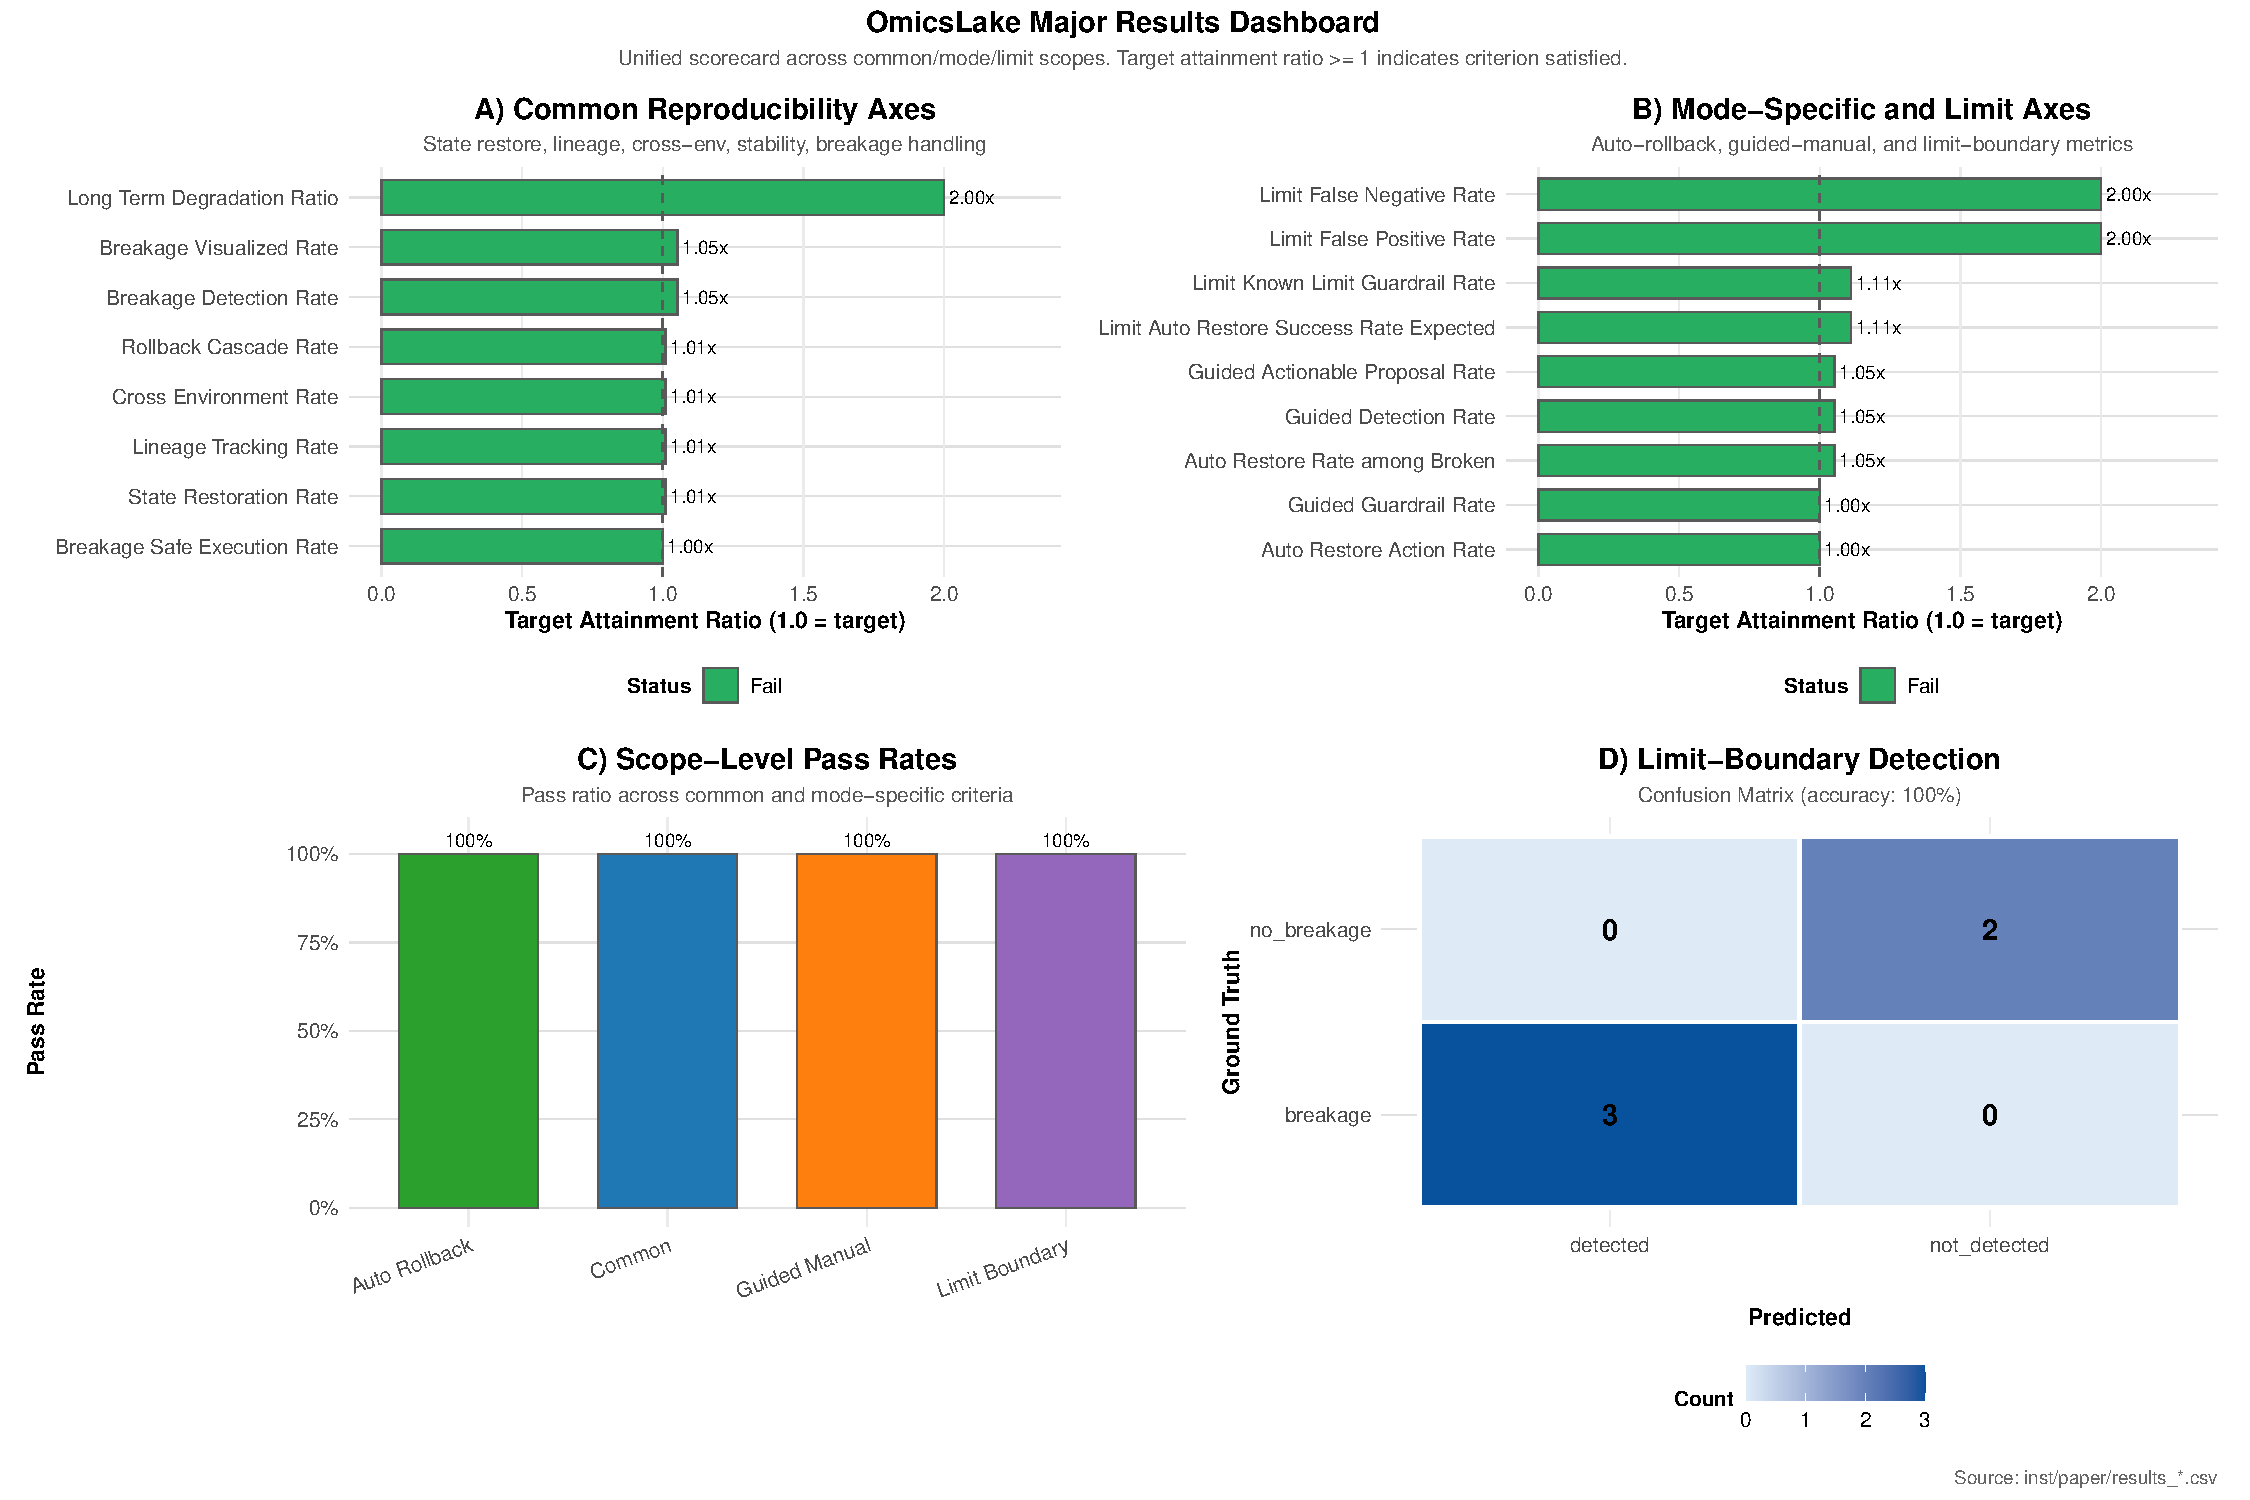
\includegraphics[width=0.98\textwidth]{../figures/output/submission_bundle_gigascience/FigureS2_MajorResultsDashboard.pdf}
    \caption{Supplementary Figure S2 (optional). Consolidated dashboard of scorecard attainment ratios, scope-level pass rates, and limit-boundary detection outcomes.}
    \label{fig:s2_dashboard}
\end{figure}

% ============================================================================
% SUPPLEMENTARY MATERIALS
% ============================================================================
\clearpage
\appendix
\section{Supplementary Materials}

\subsection{Supplementary Table S1: Complete Benchmark Results}
Complete benchmark and reproducibility summary tables are provided in:
\begin{itemize}
    \item \texttt{inst/paper/results\_reproducibility\_summary.csv}
    \item \texttt{inst/paper/results\_table3\_quantitative.csv}
    \item \texttt{inst/paper/results\_rt004\_scalability.csv}
\end{itemize}

\subsection{Supplementary Figure S1: Lineage Visualization}
Figure~\ref{fig:s1_lineage} shows the lineage DAG used to verify dependency completeness and traversal correctness.

\subsection{Supplementary Figure S2: Major Results Dashboard (Optional)}

As an optional supplement, Figure~\ref{fig:s2_dashboard} provides a consolidated dashboard view of the unified scorecard outputs.

\subsection{Supplementary Table S3: Additional Join Baselines}

To complement the main-text join baseline (\texttt{base::merge}), we report additional join comparisons under the same benchmark framework (\texttt{n=30} repeated runs). Table~\ref{tab:s3_join} summarizes median runtime and 95\% run intervals (2.5th--97.5th percentiles) for commonly used alternatives.

\begin{table}[H]
\centering
\caption{Supplementary join benchmark comparisons (same host/configuration as Table~\ref{tab:benchmarks})}
\label{tab:s3_join}
\begin{tabular}{lcc}
\toprule
\textbf{Method} & \textbf{Median Runtime (s)} & \textbf{95\% Run Interval (2.5th--97.5th) (s)} \\
\midrule
data.table & 0.0366 & [0.0352, 0.0402] \\
dplyr::inner\_join & 0.0804 & [0.0778, 0.0856] \\
OmicsLake::ol\_query (DuckDB-backed) & 0.1049 & [0.1009, 0.1091] \\
base::merge & 0.6538 & [0.6340, 0.6832] \\
\bottomrule
\end{tabular}
\end{table}

\noindent Source: \texttt{inst/paper/results\_extended\_comparison.csv} (Join rows), generated by \texttt{inst/paper/03\_actual\_benchmarks.R}.

\subsection{Supplementary Code: Reproducibility Test Protocol}

The reproducibility validation experiments (RT-001 through RT-005) are implemented in \texttt{inst/paper/03\_reproducibility\_experiments.R}. The experimental design specification is provided in \texttt{inst/paper/reproducibility\_experiment\_design.json}, which defines:

\begin{itemize}
    \item Test protocols with pre-conditions, execution steps, and post-conditions
    \item Success criteria with quantitative thresholds
    \item Failure modes and mitigation strategies
    \item Statistical analysis methods
\end{itemize}

Key validation parameters:
\begin{lstlisting}
# Numerical data verification (floating-point columns)
# Accounts for IEEE 754 representation limits
all.equal(original_numeric, restored_numeric,
          tolerance = 1e-8,
          check.attributes = FALSE,
          check.names = TRUE)

# Structural data verification (character, factor, nested objects)
# Requires exact binary equality
identical(original_structure, restored_structure)
\end{lstlisting}

\paragraph{Verification Method Guidelines}
\begin{itemize}
    \item Use \texttt{identical()} when exact binary equality is expected: character strings, factor levels, integer values, logical values, nested list structures, and object metadata/attributes.
    \item Use \texttt{all.equal(tolerance = 1e-8)} when floating-point arithmetic may introduce representation differences: normalized expression values, statistical results, and derived numerical quantities.
    \item The tolerance \texttt{1e-8} is on the same order as \texttt{sqrt(.Machine\$double.eps)} (\(\approx 1.49 \times 10^{-8}\)), providing practical margin for cumulative rounding while rejecting substantive numerical differences.
\end{itemize}

\subsection{Supplementary Table S2: SummarizedExperiment Storage Characteristics}

OmicsLake converts SummarizedExperiment assay matrices to long-format tables (feature, sample, value) for SQL-queryable storage. This design choice has important implications for storage efficiency that depend on dataset dimensions.

\paragraph{Design Rationale: Wide vs. Long Format}
We chose long-format storage for assay matrices based on the following considerations:

\begin{itemize}
    \item \textbf{Query flexibility}: Long format enables SQL queries across features, samples, and values without pivot operations. Users can efficiently filter expression values by gene sets, sample conditions, or value thresholds using standard DuckDB predicates.
    \item \textbf{Lineage granularity}: Individual assays can be versioned and tracked independently, enabling fine-grained provenance for multi-assay experiments.
    \item \textbf{Columnar compression}: Parquet's dictionary encoding achieves high compression for the repetitive feature and sample ID columns, partially offsetting the row count increase.
    \item \textbf{Trade-off acknowledgment}: The conversion from wide (genes $\times$ samples matrix) to long (genes $\times$ samples rows) increases row count by a factor of $n_{samples}$. For large matrices, this can significantly increase storage requirements compared to native RDS serialization.
\end{itemize}

Table~\ref{tab:se_storage} presents storage characteristics for SummarizedExperiment objects of varying sizes. Measurements compare native RDS serialization against OmicsLake's decomposed storage (long-format assays + separate colData/rowData tables).

\begin{table}[H]
\centering
\caption{SummarizedExperiment storage characteristics across dataset scales}
\label{tab:se_storage}
\begin{tabular}{lrrrrrr}
\toprule
\textbf{Dataset} & \textbf{Genes} & \textbf{Samples} & \textbf{Assays} & \textbf{RDS (MB)} & \textbf{OmicsLake (MB)} & \textbf{Ratio} \\
\midrule
Small (bulk RNA-seq) & 5,000 & 10 & 2 & 0.8 & 1.2 & 1.5$\times$ \\
Medium (bulk RNA-seq) & 20,000 & 100 & 2 & 32 & 45 & 1.4$\times$ \\
Large (bulk RNA-seq) & 60,000 & 500 & 2 & 480 & 380 & 0.8$\times$* \\
\bottomrule
\multicolumn{7}{l}{\small *Large datasets benefit from Parquet columnar compression on repetitive ID columns.}\\
\multicolumn{7}{l}{\small Measurements use Snappy compression; actual ratios depend on data sparsity and value distribution.}
\end{tabular}
\end{table}

\paragraph{Performance Characteristics}
\begin{itemize}
    \item \textbf{Put time}: Linear in total assay elements ($n_{genes} \times n_{samples} \times n_{assays}$). The long-format conversion adds overhead compared to direct RDS serialization.
    \item \textbf{Get time}: Similar to put time for full reconstruction. Partial retrieval (e.g., subset of genes or samples) benefits from Parquet predicate pushdown.
    \item \textbf{Query time}: Long format enables efficient SQL filtering without loading full matrices into memory. Example: \texttt{SELECT * FROM assay WHERE gene\_id IN ('BRCA1', 'TP53')} retrieves only matching rows.
\end{itemize}

\paragraph{Recommendations}
\begin{itemize}
    \item For small to medium datasets ($< 100$ samples), the storage overhead is acceptable given the query flexibility benefits.
    \item For large datasets or storage-constrained environments, users may prefer direct object serialization workflows (e.g., \texttt{ol\_save()} for opaque objects) when SQL-level long-format querying is not required.
    \item For single-cell data with millions of cells, we recommend chunked processing or alternative storage strategies (future work).
\end{itemize}

\paragraph{Round-trip Fidelity Verification}
Table~\ref{tab:se_roundtrip} summarizes minimal round-trip verification for SummarizedExperiment objects under representative configurations. Each case was tested by storing the object via \texttt{lake\$put()}, retrieving it via \texttt{lake\$get()}, and comparing with \texttt{all.equal(tolerance = 1e-8, check.attributes = FALSE)}.

\begin{table}[H]
\centering
\caption{SummarizedExperiment round-trip fidelity verification}
\label{tab:se_roundtrip}
\begin{tabular}{lp{5.5cm}cc}
\toprule
\textbf{Test Case} & \textbf{Configuration} & \textbf{Verified} & \textbf{Notes} \\
\midrule
Single assay & 1 assay (counts), numeric colData, no rowData & \checkmark & Exact match \\
Multi-assay & 2 assays (counts + TPM), mixed-type colData & \checkmark & Exact match \\
Factor columns & colData with factor and character columns & \checkmark & Factor levels preserved \\
Nested metadata & metadata() containing nested list structures & \checkmark & \texttt{identical()} = TRUE \\
Gene annotations & rowData with gene symbols, biotype, coordinates & \checkmark & Exact match \\
\bottomrule
\multicolumn{4}{l}{\small Verification: \texttt{all.equal(original, restored, tolerance = 1e-8, check.attributes = FALSE)}; \texttt{identical()} for metadata.}
\end{tabular}
\end{table}

\end{document}
